\documentclass[a4paper,12pt]{article}


\usepackage{enumitem}
\usepackage{graphicx}
\pagestyle{empty}
\begin{document}

\begin{center}
\huge{MAT013: Module plan}
\end{center}
\begin{center}
\tiny{(This sheet was last updated on \today)}
\end{center}

\section{Description}
This plan is a description of the teaching methodologies for the entire MAT013 module. This module aims to teach students how to use two statistical packages: SAS and R and is taught over 4 morning long periods over 4 weeks as shown in Figures \ref{chapter} and \ref{Days}.

\begin{figure}[htdp]
    \begin{center}
        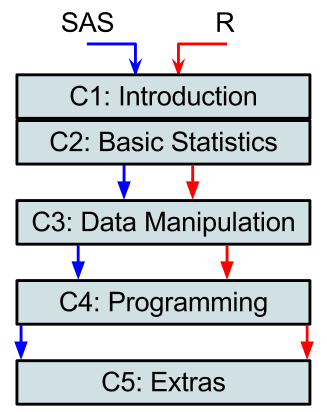
\includegraphics[width=6cm]{images/chapters.png}
    \end{center}
    \caption{Outline of the course}
    \label{chapter}
\end{figure}

\begin{figure}[htdp]
    \begin{center}
        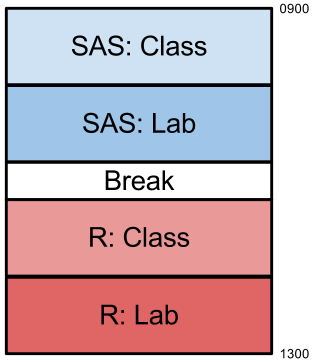
\includegraphics[width=6cm]{images/Days.png}
    \end{center}
    \caption{Day schedule}
    \label{Days}
\end{figure}

The course will be taught in a non traditional way use various forms of pre-class (non-contact time) instruction as well as a peer lead inquiry based learning approach. This methodology is justified in my PCUTL covering claim and based on a thorough investigation of the literature.\\

Figure \ref{Module_plan} summarises the proposed approach.

\begin{figure}[htdp]
    \begin{center}
        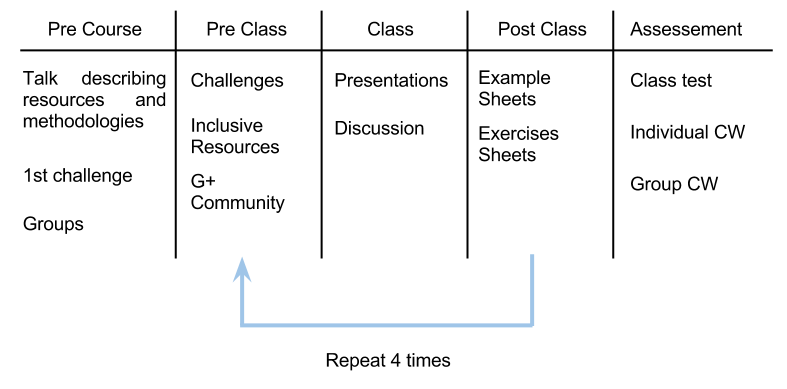
\includegraphics[width=12cm]{images/Module_plan.png}
    \end{center}
    \caption{Summary of module approach.}
    \label{Module_plan}
\end{figure}


\section{Discussion}
I will here discuss in detail how the above approach relates to issues of:

\begin{itemize}
    \item Inclusivity;
    \item Contact and non-contact time teaching;
    \item Technology enhanced education.
\end{itemize}

\subsection{Inclusivity}

Various issues of inclusivity have been taken in to account:

\begin{itemize}
    \item All data sets have been carefully considered to avoid issues of heteronomality, gender biais and/or religion;
    \item All teaching rooms used are fitted with inductive audio loops;
    \item There are no issues related to access to the various teaching rooms required;
\end{itemize}

The student groups (already assigned) have taken in to account various aspects of the literature (again these are detailed in my covering claim), ensuring a mix of age, gender and cultural heritage. Importantly, the MSc does quite a lot of group activity and so these groups are purposefully aiming to build on strong relationships but also encourage new ones.\\

The use of videos in a flipped classroom approach also enters in to the realm of inclusivity as the videos can be viewed easily on most platforms. Furthermore, the videos cover the entirety of the course contents (approximately 4 hours of videos) and should enable students to overcome issues of communication by viewing the videos at their own pace.\\

Finally all teaching materials have been written in markdown and translated via pandoc in to various formats:

\begin{itemize}
    \item .pdf
    \item .md
    \item .html
    \item .docx
\end{itemize}

The first 3 formats of the documents ensure that students will be able to read the content on any operating system and/or platform without loss of formatting etc. The last 3 formats ensure that students can if need be change the font and/format of the notes as desired.  This holds for all teaching materials involved (example sheets etc...).  \\

Furthermore, at the first discussion with the students (``pre class'') I will remind them to let me know if there are any other issues relating to inclusivity.\\

Finally, all materials will be distributed to students using my personal website, ensuring once again ease of access.

\subsection{Contact and non contact-time teaching}

The course is designed to involve a large amount of non-contact time teaching. This is scaffolded using various technological solutions including:

\begin{itemize}
    \item Challenges;
    \item Videos;
    \item Full set of notes;
    \item An online community.
\end{itemize}

The challenge sheet is the main focus of the non-contact time teaching. In groups, students will be expected to work on a particular challenge in their own time. In class (i.e. during contact time) students will present their solutions to their peers and a further discussion will arise. The challenges are designed in such a way as to guide students towards their ILOs but if these are missed I will be able to step in a discuss any particular subject as necessary.\\

The various resources available to the students are meant to be helpful (and indeed contain all the necessary content) but students will be encouraged to find other resources and also communicate as necessary. To aid with this, a community on Google plus has been setup.\\

Finally a copy of the notes will be made available to the students on Google Docs to encourage the students to make amendments, and/or include other examples.\\

\subsection{Technology enhanced education}

Technology is used throughout this teaching plan to enhance the learning of students. Most of the aspects have been touched on above but here is a summary:

\begin{itemize}
    \item Multiple short videos (approximately 5 minutes in length) have been designed covering all aspects of the course;
    \item Notes are translated in to most available formats using pandoc;
    \item A copy of the notes is being made available in google docs for online collaboration of students;
    \item A google plus community has been setup to encourage students to take ownership of the course content.
\end{itemize}

It is firmly felt that the use of technology is justified in this course.

\end{document}
